\chapter{Grundlagen}

Im folgenden Kapitel sollen die für das Verständnis der weiteren Arbeit benötigten Grundlagen geschaffen werden. Dazu soll zunächst die im vorherigen Kapitel informell beschriebene zielorientierte Interaktion des Agenten mit seiner Umgebung einen formalen Rahmen erhalten. Hierfür eignet sich als theoretisches Grundgerüst der Markov-Entscheidungs-Prozess (MDP). Dieser stellt einen Formalismus für sequentielle Entscheidungsprobleme dar und ermöglicht die Definition weiterer grundlegender Begriffe des \ac{RL} wie beispielsweise der Policy und der State-Value Funktion. Insbesondere lässt sich das Lernziel bzw. das Optimierungsproblem mithilfe des MDP formal ausdrücken. Im nächsten Abschnitt werden die Funktionsweise des in dieser Arbeit verwendeten Lernalgorithmus und die von ihm verwendete Verlustfunktion erklärt. Bei diesem handelt es sich um den Proximal Policy Optimization Algorithmus und er stellt ein Verfahren zur approximativen Lösung des zuvor beschriebenen Optimierungsproblems dar. Hierzu bestimmt er die Parameter eines Modells, welches wiederum das Verhalten des Agenten steuert. Im Rahmen dieser Arbeit basiert das Modell des Agenten auf der Neural Map. Demzufolge wird diese anschließend ausführlich erörtert. Den Abschluss des Kapitels bildet eine kurze Erklärung des Long Short-Term Memory, das in den Experimenten dieser Arbeit als Referenz für die Neural Map verwendet wird.


\section{Grundlegende Begriffe}
\label{sec_basics}

Die Definitionen des folgenden Abschnitts sind im Wesentlichen aus \cite{SuttonBarto} entnommen. Der interessierte Leser sei auf dieses Standardwerk des Reinforcement Learnings verwiesen für tiefergehende Informationen.

Der Markov-Entscheidungs-Prozess ist ein Tupel $(\mathcal{S, A}, p, r)$. Dabei ist $\mathcal{S}$ die Menge der Zustände, auch Zustandsraum genannt. Mit $\mathcal{A}$ wird die Menge der Aktionen bzw. der Aktionsraum bezeichnet. Das Verhalten der Umgebung wird durch die Zustands-Übergangs-Wahrscheinlichkeit $p: \mathcal{S} \times \mathcal{S} \times \mathcal{A} \to [0,1]$ beschrieben. So gibt $p(s'|s,a)$ die Wahrscheinlichkeit dafür an, dass die im Zustand $s$ ausgeführte Aktion $a$  zum Folgezustand $s'$ führt. Mit jedem dieser Zustands-Übergänge ist ein Reward verknüpft, der durch die Reward-Funktion $r: \mathcal{S} \times \mathcal{A} \times \mathcal{S} \to \mathbb{R}$ spezifitiert wird.

Die Interaktion des Agenten mit der Umgebung findet zu diskreten Zeitpunkten $t = 0, 1, 2, 3,\dots$ statt. Er erhält zu jedem Zeitpunkt $t$ von der Umgebung deren aktuellen Zustand $s_t \in \mathcal{S}$. Dieser bildet die Entscheidungsgrundlage für die Auswahl der Aktion $a_t \in \mathcal{A}$ durch den Agenten. Die Umgebung widerum gibt dem Agenten im nächsten Zeitschritt $t+1$ als Reaktion auf die zuvor ausgewählte Aktion eine Belohnung $R_{t+1}$ und präsentiert ihm den Folgezustand $s_{t+1}$. Auf Basis dessen wählt der Agent die nächste Aktion $a_{t+1}$ aus, erhält den Reward $r_{t+2}$, u.s.w. Die Abbildung \ref{fig_schnittstelle} verdeutlicht diese Interaktion zwischem dem Agenten und der Umgebung. Die auf diese Weise entstehende Sequenz $s_0, a_0, R_{t+1}, s_{t+1}, a_{t+1}, R_{t+2}, s_{t+2}, a_{t+2}, R_{t+3},\dots$ wird auch als Trajektorie bezeichnet. Wenn sich die Interaktion des Agenten mit der Umgebung infolge der ihm gestellten Aufgabe in Subsequenzen unterteilen lässt, wird von einer episodischen Aufgabe gesprochen. Beispiele hierfür sind Computerspiele oder das Finden von Wegen aus Labyrinthen. Die dabei entstehenden Trajektorien endlicher Länge werden Episoden genannt und ihr letzter Zustand heißt Terminalzustand $s_T$. Mit Erreichen eines solchen wird die Umgebung zurückgesetzt in einen Anfangszustand und es beginnt eine neue Episode. Es kann einen oder mehrere Terminalzustände geben und es ist sichergestellt, dass der Agent einen dieser Terminalzustände erreichen kann bzw. wird. Es sei an dieser Stelle angemerkt, dass die im Rahmen dieser Arbeit durchgeführten Experimente allesamt aus episodischen Aufgaben bestehen.

\begin{figure}[ht!]
  \centering
  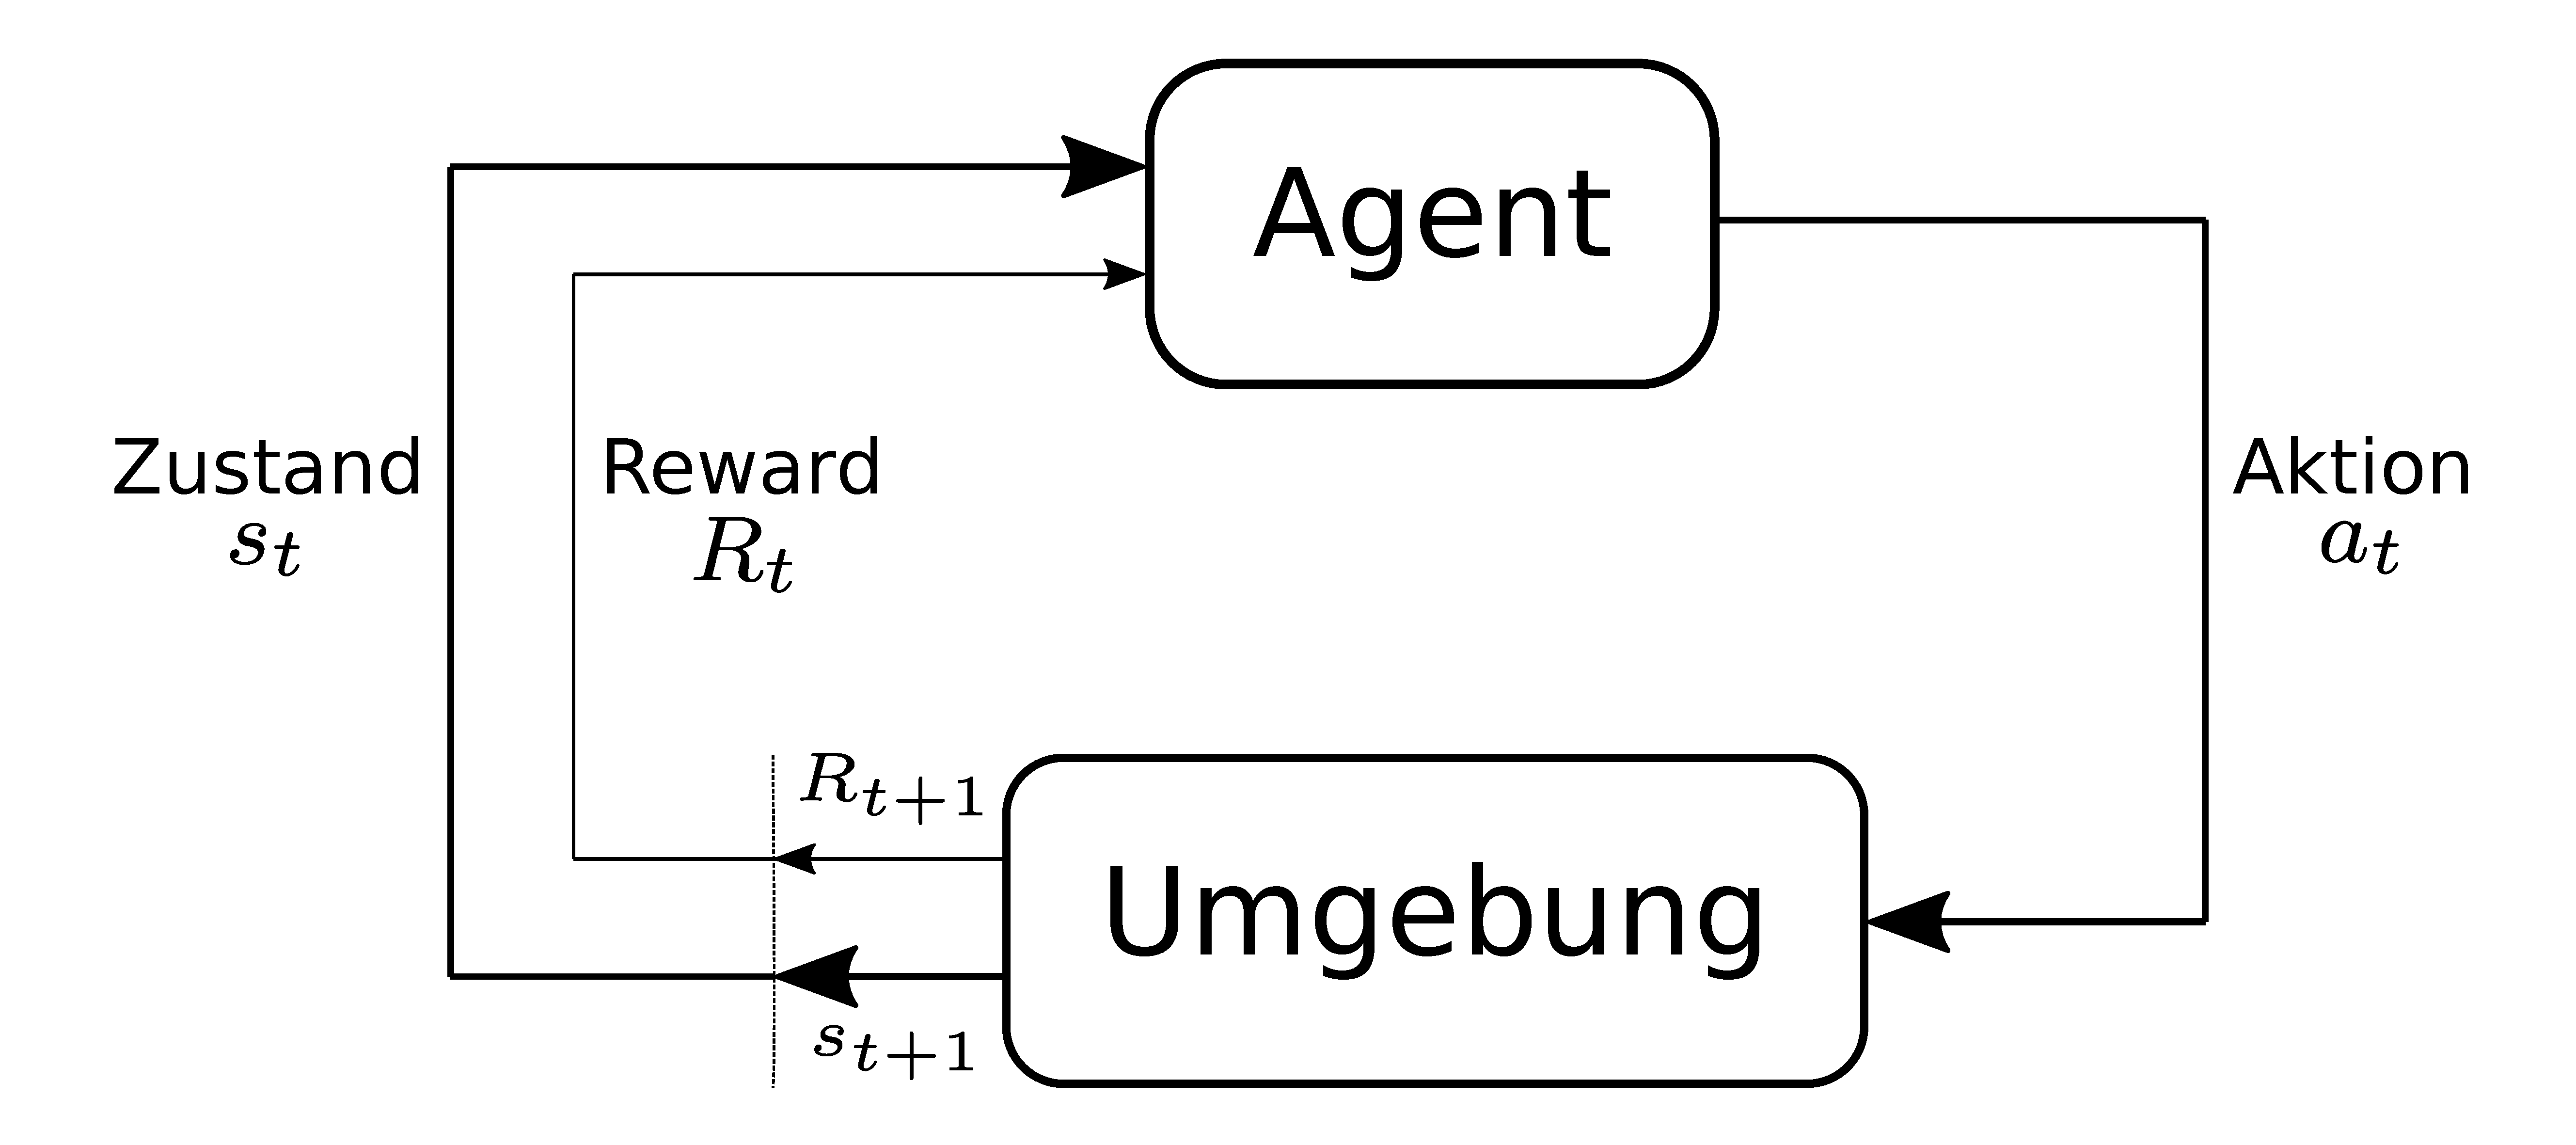
\includegraphics[keepaspectratio,width=0.75\textwidth]{abbildungen/schnittstelle_agent_umgebung.pdf}
  %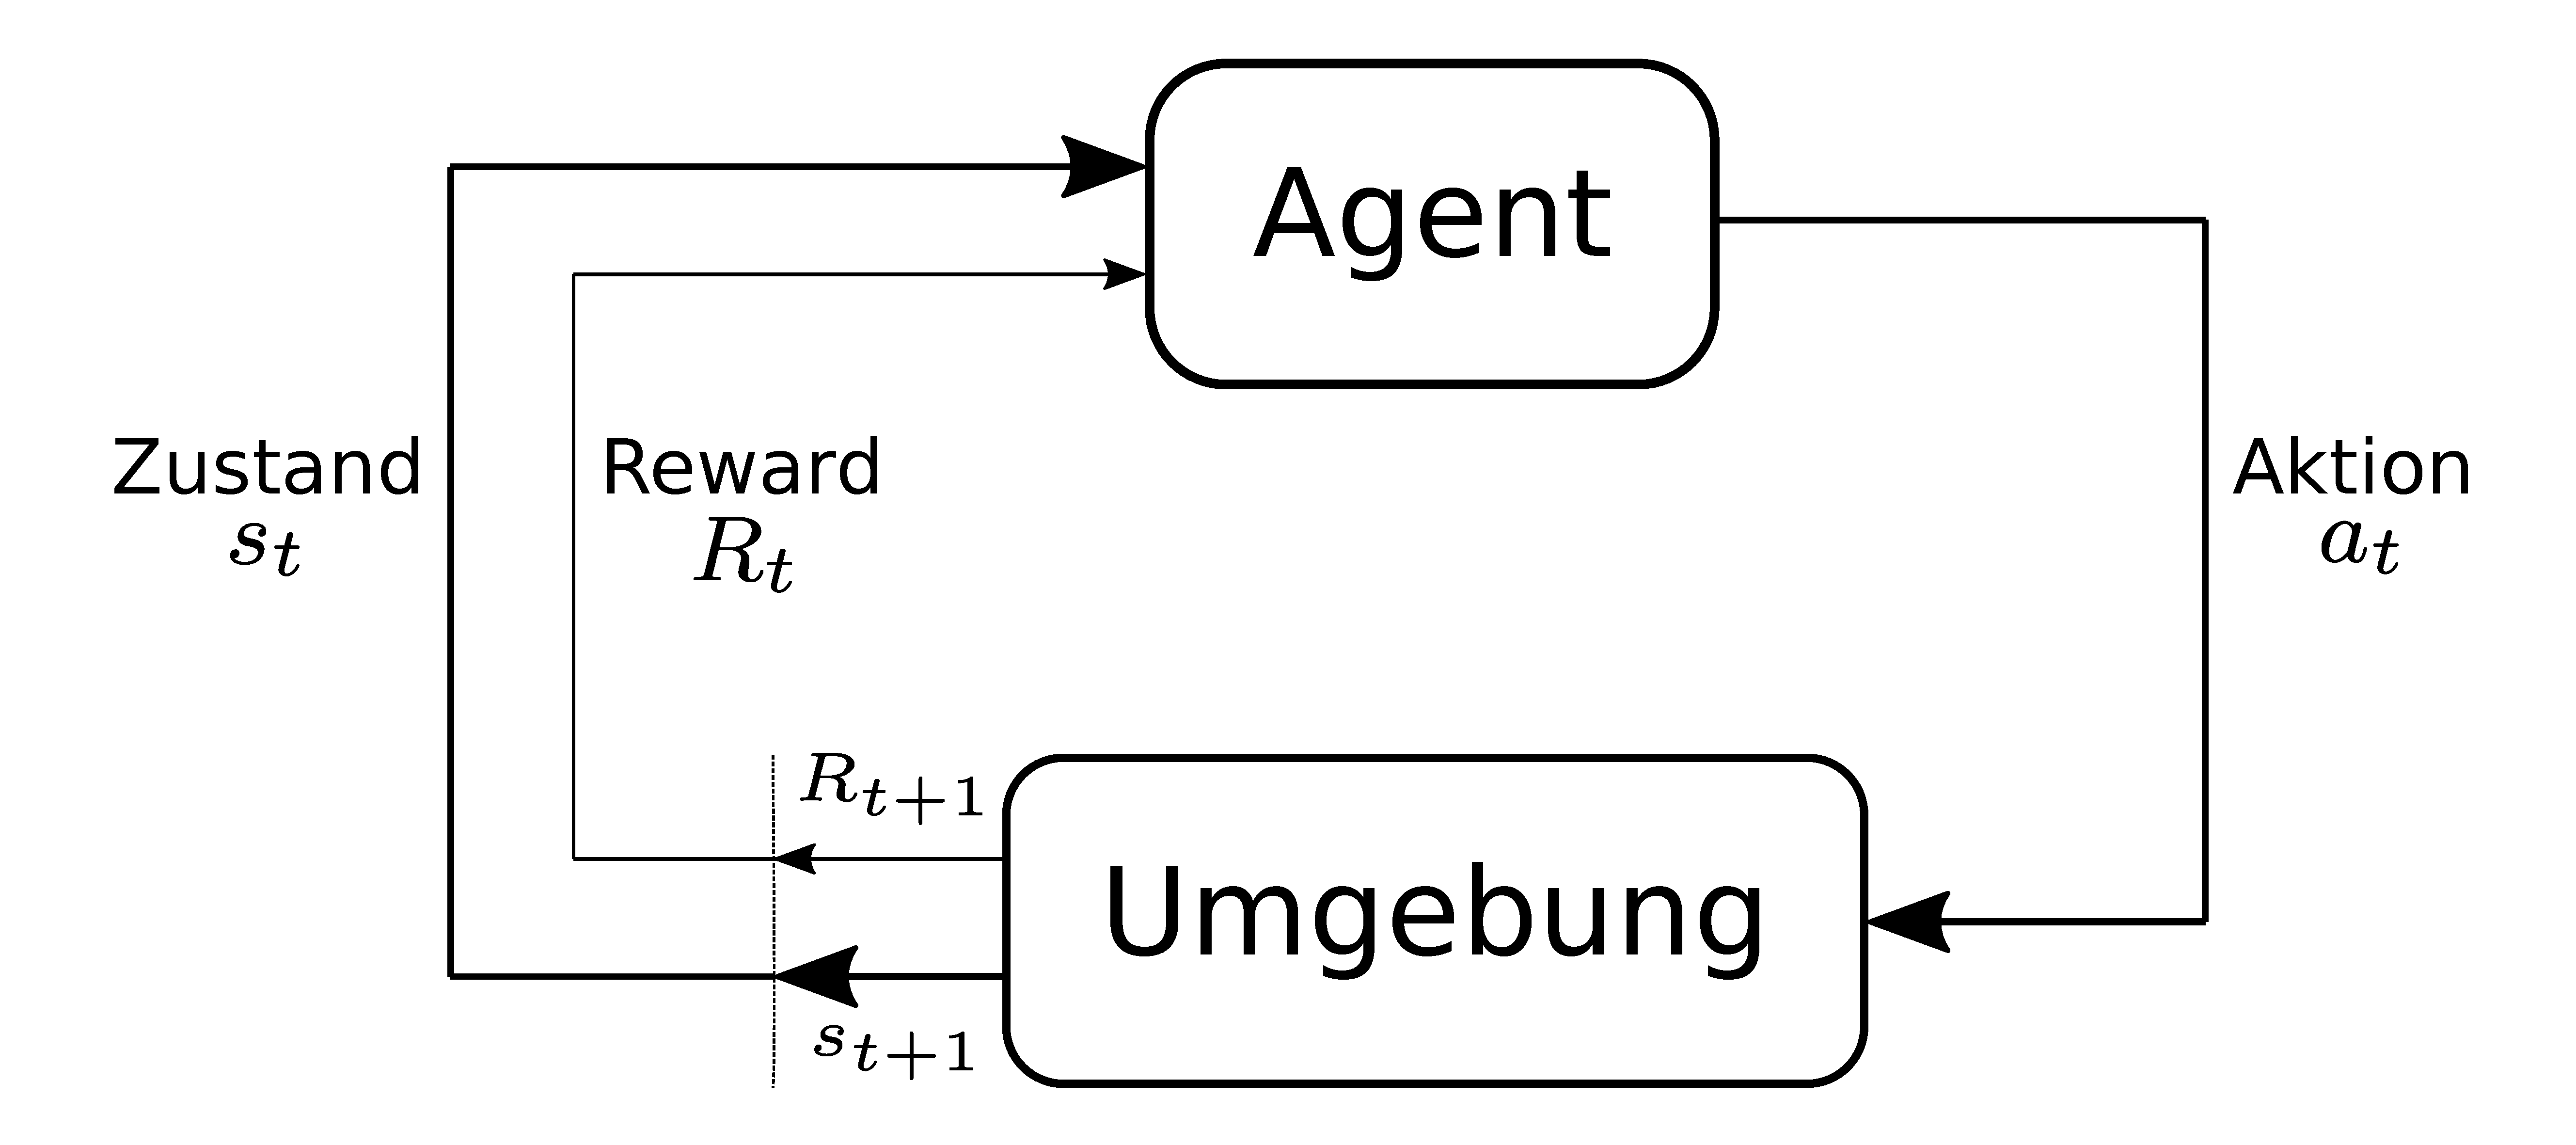
\includegraphics[height=0.5\textwidth, width=0.9\textwidth]{abbildungen/schnittstelle_agent_umgebung.pdf}
  \caption{Die Abbildung zeigt die Interaktion zwischen dem Agenten und der Umgebung, d.h. die Auswahl einer Aktion durch den Agenten basierend auf einem Zustand und die Reaktion der Umgebung in Form eines Rewards und eines Folgezustands.}
  \label{fig_schnittstelle}
\end{figure}

Das Ziel des Agenten beim Reinforcement Learning besteht darin, in jedem Zeitschritt seine Aktion so auszuwählen, dass die Gesamtmenge der vom ihm erhaltenen Belohnungen maximiert wird. Um dieses informelle Ziel zu formalisieren, wird der discounted Return $G_t$ zum Zeitpunkt $t$ definiert als

\begin{equation}
  G_t = R_{t+1} + \gamma R_{t+2} + \gamma R_{t+3} + \dotsb = \sum_{k=0}^{\infty} \gamma^k R_{t+k+1},
  \label{return_eq}
\end{equation}

wobei $\gamma \in [0, 1]$ als discount Faktor bezeichnet wird. Dieser regelt, wie stark zukünftige Rewards berücksichtigt werden. So ist ein Reward, der erst in $k$ Zeitschritten erhalten wird, um den Faktor $\gamma^{k-1}$ weniger Wert im Vergleich zu einem unmittelbar erhaltenen. Praktisch gesehen wird auf diese Art und Weise die Kurz- bzw. Weitsichtigkeit des Agenten reguliert. Im Falle episodischer Aufgaben vereinfacht sich die unendliche Summe aus Gleichung \eqref{return_eq} zu einer endlichen Summe. Dabei ist die obere Summationsgrenze $T$, d.h. der Zeitschritt des Terminalzustands $s_T$. Des Weiteren besitzt der Return die rekursive Eigenschaft $G_t = R_{t+1} + \gamma G_{t+1}$, welche für nachfolgende Definitionen von erheblicher Wichtigkeit ist.

Zum Erreichen seines Lernziels muss der Agent ein entsprechendes Verhalten erlernen, d.h. er muss für jeden Zustand $s_t$ die Aktion $a_t$ kennen, sodass schlussendlich die Summe der Belohnungen maximal wird. Zur Formalisierung des Verhaltens des Agenten, also der Auswahl von Aktionen unter Berücksichtigung des aktuellen Zustands, wird die sogenannte Policy $\pi: \mathcal{A} \times \mathcal{S} \to [0, 1]$ definiert. Dabei ist $\pi(s|a)$ eine Wahrscheinlichkeitsverteilung über alle möglichen Aktionen $a$ unter der Bedingung, dass sich die Umgebung im Zustand $s$ befindet. Zu Beginn des Lernprozesses wird die Policy für gewöhnlich zufällig initialisiert. Anschließend wird sie schrittweise solange verändert, bis keine Verbesserung mehr auftritt. Hat der Agent an diesem Punkt die ihm gestellte Aufgabe erfolgreich gelöst, ist dies in der Regel gleichbedeutend damit, dass er die optimale Policy oder eine Approximation selbiger erlernt hat. In der Zukunft kann er dann zur Bewältigung dieser Aufgabe einfach für jeden Zustand die Aktion mit der größten Wahrscheinlichkeit auswählen.

Um die Auswahl der aktuellen Aktion $a_t$ möglichst sinnvoll vorzunehmen, werden neben dem aktuellen Zustand $s_t$ auch Informationen darüber benötigt, inwiefern die aktuelle Entscheidung zukünftige Rewards beeinflusst. Nur so ist es dem Agenten möglich, die längerfristigen Folgen seines aktuellen Handelns abzuschätzen und somit die Summe über alle erhaltenen Rewards zu maximieren und nicht nur den Aktuellen. Der Agent würde also gerne wissen, \glqq wie gut \grqq{} es bezüglich zukünftiger Rewards ist, sich in einem bestimmen Zustand zu befinden bzw. eine bestimmte Aktion in einem bestimmten Zustand auszuführen. Zusammen mit der zuvor eingeführten Policy, die das zukünftige Verhalten des Agenten steuert, lassen sich entsprechende Bewertungsfunktionen definieren, die darüber Aufschluss geben. Hierzu wird eine State-Value Funktion wie folgend definiert:

\begin{equation*}
  v_\pi(s) = \mathbb{E}_\pi[G_t|s_t=s] = \mathbb{E}_\pi[\sum_{k=0}^{\infty} \gamma^k R_{t+k+1} | s_t=s], \quad \forall s \in \mathcal{S}
  \label{v_pi_eq}
\end{equation*}

Die State-Value Funktion eines Zustands $s$ für eine Policy $\pi$ entspricht dem erwarteten Return, der sich ergibt, wenn der Agent im Zustand $s$ startet und ab dort der Policy $\pi$ folgt, d.h. seine Aktionen basierend auf $\pi(a|s)$ auswählt. Dabei ist der Wert eines Terminalzustandes als Null definiert. Auch die State-Value Funktion verfügt über eine rekursive Eigenschaft, die widerum aus der des Returns resultiert. Die folgende Gleichung setzt den Wert des aktuellen Zustands $s$ in Beziehung zu den Werten möglicher Folgezustände $s'$ und wird als Bellmann-Gleichung für $v_\pi$ bezeichnet:

\begin{equation}
  v_\pi(s) = \mathbb{E}_\pi[R_{t+1} + \gamma G_{t+1} | s_t=s] = \sum_{a} \pi(a|s) \sum_{s'} p(s'|s,a) [r(s,a,s') + \gamma v_\pi(s')]
  \label{v_pi_bellmann_eq}
\end{equation}

Die Berechnung des Erwartungswertes kann sich dabei wie folgend vorgestellt werden. Zunächst werden die im Zustand $s$ möglichen Aktionen $a$ mit der auf der Policy $\pi(a|s)$ beruhenden Auftrittswahrscheinlichkeit gewichtet. Somit entstehen konkrete Auswahlen von $s$ und $a$. Hieraus wiederum resultieren Folgezustände $s'$, die ihrerseits mit der Zustands-Übergangs-Wahrscheinlichkeit $p(s'|s,a)$ gewichtet werden. Auf diese Art und Weise erhält jeder Summand, d.h. der Inhalt der Klammern für eine konkrete Wahl von $s$, $a$ und $s'$, seine eigene Gewichtung. Abschließend wird dann über alle entsprechend gewichtetet Möglichkeiten aufsummiert. Die Bellmann-Gleichung für $v_\pi$ bildet die theoretische Grundlage für viele Verfahren, die die State-Value Funktion erlernen. Im denkbar einfachsten Verfahren wird $v_\pi$ schrittweise berechnet, indem die rechte Seite von Gleichung \eqref{v_pi_bellmann_eq} als Update-Regel verwendet wird. Hierzu muss allerdings $p(s'|s,a)$ bekannt sein, was jedoch oftmals nicht der Fall ist.

Analog zu $v_\pi$ lässt sich die sogenannte Action-Value Funktion $q(s,a) = \mathbb{E}_\pi[G_t | s_t=s, a_t=a]$ definieren. Diese gibt den erwarteten Return an für den Fall, dass der Agent im Zustand $s$ die Aktion $a$ tätigt und ab da an der Policy $\pi$ folgt. Sie erlaubt somit eine Bewertung einer bestimmten Aktion in einem bestimmen Zustand unter Berücksichtigung einer Policy.

Da State-Value Funktionen die Möglichkeit bieten, eine Ordnung auf den Policys zu definieren, lässt sich eine optimale Policy auf die folgende Art und Weise definieren. Eine Policy $\pi$ ist besser oder gleich als eine policy $\pi'$, wenn der erwartete Return von $\pi$ für alle Zustände größer oder gleich ist als der von $\pi'$, d.h. $\pi \ge \pi'$, wenn $v_\pi(s) \ge v_{\pi'}$ für alle $s \in \mathcal{S}$. Es gibt immer mindestens eine Policy die besser als oder zumindest gleich ist im Vergleich zu allen anderen Policys. Dies ist die optimale Policy und sie wird mit $\pi_*$ bezeichnet. Die optimale State-Value Funktion $v_*$ wird definiert als $v_*(s) = max_\pi v_\pi(s)$ für alle $s \in \mathcal{S}$.

Ein Agent, dem es gelungen ist, die optimale Policy bzw. State-Value Funktion zu lernen, hat die ihm gestellte Aufgabe logischerweise im bestmöglichen Sinne gelöst. Leider tritt dieser Fall in der Realität so gut wie nie auf, sondern es sind in der Regel nur approximative Lösungen für die Policy bzw. State-Value Funktion möglich. Ursächlich hierfür sind hauptsächlich zwei Gründe. Zum einen ist die Zustands-Übergangs-Wahrscheinlichkeit $p(s'|s,a)$ oftmals nicht bekannt und zum anderen überschreitet der Rechenaufwand zur Bestimmung der optimalen Policy bzw. State-Value Funktion in der Regel die verfügbaren Ressourcen. So sind beispielsweise die Zustandsräume so groß, dass es aus Gründen der zur Verfügung stehenden Speichermenge unmöglich ist, für jeden Zustand $s$ den Wert von $v(s)$ vorzuhalten. In der Folge werden dann Funktionsapproximatoren wie beispielsweise Neuronale Netze für die eingesetzt, um die Policy und/oder die State-Value Funktion geeignet zu schätzen. Um die Parameter eines solchen Modells geeignet zu trainieren, wird ein entsprechender Lernalgorithmus benötigt. Dieser wird im nächsten Abschnitt präsentiert.


\section{Proximal Policy Optimization}
\label{sec_ppo}

Für die im weiteren Verlauf dieser Arbeit durchgeführten Experimente wird der \ac{PPO} Algorithmus verwendet. Dieser wurde von J. Schulman et. al. im Jahr 2017 veröffentlicht \cite{PPO}. Grundsätzlich handelt es sich bei \ac{PPO} um eine Policy Gradientenmethode und im Speziellen um ein sogenanntes Actor-Critic Verfahren. Policy Gradientenmethoden sind in der Lage eine parametrisierte Policy zu erlernen, wie sie im Rahem dieser Arbeit benutzt werden soll. Dazu wird ein skalares Leistungsmaß unter Berücksichtigung der Policy Parameter definiert, welches anschließend maximiert wird, indem ein Gradientenaufstieg durchgeführt wird. Actor-Critic Verfahren erweitern dieses Vorgehen. Die Policy, die die Auswahl der Aktionen vorgibt, wird als Actor bezeichnet. Der Critic bewertet die zuvor vom Actor ausgewählten Aktionen. Dazu erlernt er beispielsweise die State-Value Funktion. Auf Basis der Bewertung des Critics verbessert der Actor die Policy. Somit ist der grundlegende Ablauf von \ac{PPO} folgender. Durch eine Interaktion mit der Umgebung, d.h. basierend auf der Policy werden Aktionen ausgewählt und ausgeführt, werden Daten generiert. Diese werden anschließend genutzt, um unter Verwendung eines Gradientenaufstiegs die Verlustfunktion zu optimieren. Während herkömmliche Policy Gradientenmethoden nur ein Gradientenupdate pro Datenwert anwenden, haben Schulman et. al. in ihrem Paper eine neue Verlustfunktion präsentiert, die dazu geeignet ist, mehrere Trainingsepochen basierend auf denselben Daten durchzuführen. Hierdurch weißt \ac{PPO} eine erhöhte Effizienz bei der Nutzung der zum Training zur Verfügung stehenden Daten auf. Da sich gradientenbasierte Verfahren bei der Optimierung der Verlustfunktion sehr sensitiv hinsichtlich der Schrittweite verhalten, übernimmt \ac{PPO} diesbezüglich einige Vorteile des Trust Region Policy Optimization (TRPO) Algorithmus. Dieser benutzt eine Verlustfunktion, die sicherstellt, dass die nach einem Gradientenupdate erhaltene neue Policy nicht zu stark von der alten Policy abweicht und somit katastrophale Sprünge in der Performance der Policy verhindert. Allerdings erreicht TRPO dieses Ziel nur mit einem immensen Rechenaufwand, der sich entsprechend auch in einer erhöhten Komplexität bei der Implementierung niederschlägt. Dieses Problem überkommt \ac{PPO}, da er lediglich Ableitungen erster Ordnung verwendet. Des Weiteren ist \ac{PPO} sehr robust im Sinne, dass er sogut wie kein Hyperparameter-Tuning für verschiedene Lernprobleme benötigt. \\

Um die im Rahmen des \ac{PPO} Papers vorgestellte neue Verlustfunktion zu definieren, wird zunächst das Wahrscheinlichkeitsverhältnis $r_t(\theta) = \frac{\pi_\theta(a_t|s_t)}{\pi_{\theta_{old}}(a_t|s_t)}$ definiert, wobei $\pi_\theta$ die aktuelle Policy kennzeichnet und $\pi_{\theta_{old}}$ die Policy vor dem letzten Updateschritt. Somit ist $r_t(\theta)$ ein Maß dafür, wie stark sich die Wahrscheinlichkeit für die Auswahl der Aktion $a_t$ unter der Bedingung $s_t$ durch den letzten Updateschritt verändert hat. Wenn die Wahrscheinlichkeit größer geworden ist, dann ist $r_t(\theta) > 1$. Ist sie hingegen kleiner geworden, dann ist $0 < r_t(\theta) < 1$. Darüber hinaus gilt insbesondere $r(\theta_{old}) = 1$. Basierend auf $r_t(\theta)$ lässt sich eine Verlustfunktion $L^{CPI}(\theta) = \hat{\mathbb{E}}[r_t(\theta) \hat{A}_t]$ definieren. Hierbei steht CPI für conservative policy improvement und $\hat{a}_t$ ist eine Schätzung der Advantage Funktion zum Zeitpunkt $t$. Diese ist als $A(s,a) = Q(s,a) - V(s)$ definiert und gibt an wie viel besser bzw. schlechter es ist, die Aktion $a$ im Zustand $s$ auszuwählen. Die Maximierung von $L^{CPI}$ würde jedoch bei einem Updateschritt mitunter zu beliebig großen Veränderungen der Policy führen. Zur Lösung dieses Problems schlagen die Autoren folgende abgeschnittene Verlustfunktion vor:

\begin{equation}
  \label{L_CLIP}
	L^{CLIP} = \hat{\mathbb{E}}_t[min(r_t(\theta) \hat{A}_t, clip(r(\theta), 1-\epsilon, 1+\epsilon) \hat{A}_t)],
\end{equation}

wobei $\epsilon$ einen Hyperparameter beschreibt, der üblichweise aus dem Interval $[0.1, 0.2]$ stammt. Der erste Term innerhalb des Minimum-Operators ist die zuvor präsentierte Verlustfunktion $L^{CPI}$. Der zweite Term hingegen ist die abgeschnittene Variante selbiger. Der clip-Operator begrenzt den zulässigen Wertebereich von $r_t(\theta)$ auf das Interval $[1-\epsilon, 1+\epsilon]$, indem er $r_t(\theta)$ für Werte außerhalb dieses Intervals im Zweifelsfall abschneidet. Aus diesen beiden Termen wird abschließend das Minimum ausgewählt. Somit ist die Zielfunktion $L^{CLIP}$ eine untere Schranke für $L^{CPI}$. Mit dieser Methode wird eine zu große Veränderung des Wahrscheinlichkeitsverhältnisses ignoriert, wenn dadurch die Zielfunktion verbessert würde. Würde sie jedoch verschlechtert, so wird die entsprechende Veränderung inkludiert werden.

Das Verhalten der geclippten Zielfunktion \eqref{L_CLIP} wird durch Abbildung \ref{fig_L_clip} für einen einzelnen Zeitschritt $t$ verdeutlicht. Der rote Kreis entspricht dem Startpunkt der Optimierung, an dem $r = 1$ ist. Auf der linken Seite ist $L^{CLIP}$ für $A > 0$ dargestellt, d.h. die ausgeführte Aktion war besser als erwartet. Infolgedessen soll die Wahrscheinlichkeit, mit der die Aktion ausgewählt wird, erhöht werden. Um hierbei die Policy jedoch nicht zu stark zu verändern, wird $r$ bei $1+\epsilon$ geclipped. Der Fall $A < 0$ ist auf der rechten Seite abgebildet und in diesem war die ausgeführte Aktion schlechter als erwartet. Analog soll nun die dazugehörige Wahrscheinlichkeit verringert werden. Um wieder eine zu starke Veränderung der Policy zu verhindern, wird $r$ dieses mal bei $1-\epsilon$ geclipped. Die beiden zuvor angesprochenen Bereiche entsprechen dem Ignorieren einer zu großen Veränderung von $r$, wenn $L^{CLIP}$ dadurch verbessert würde. Das Inkludieren einer entsprechenden Veränderung, wenn dadurch die Zielfunktion verschlechtert würde, findet sich für $A < 0$ auf der ganz rechten Seite (und analog für $A > 0$ auf der ganz linken Seite). In diesem Fall wurde die Wahrscheinlichkeit für eine Aktion erhöht, obwohl diese schlechter als erwartet war. Somit wäre es wünschenswert, den letzten Gradientenschritt rückgängig zu machen und $L^{CLIP}$ ermöglich genau das. Die Funktion ist in diesem Bereich negativ, womit der Gradient in die entgegengesetzte Richtung zeigen wird und die Aktion im dem Maße, in dem sie zuvor wahrscheinlicher gemacht wurde, weniger wahrscheinlich machen wird.

\begin{figure}[ht!]
  \centering
  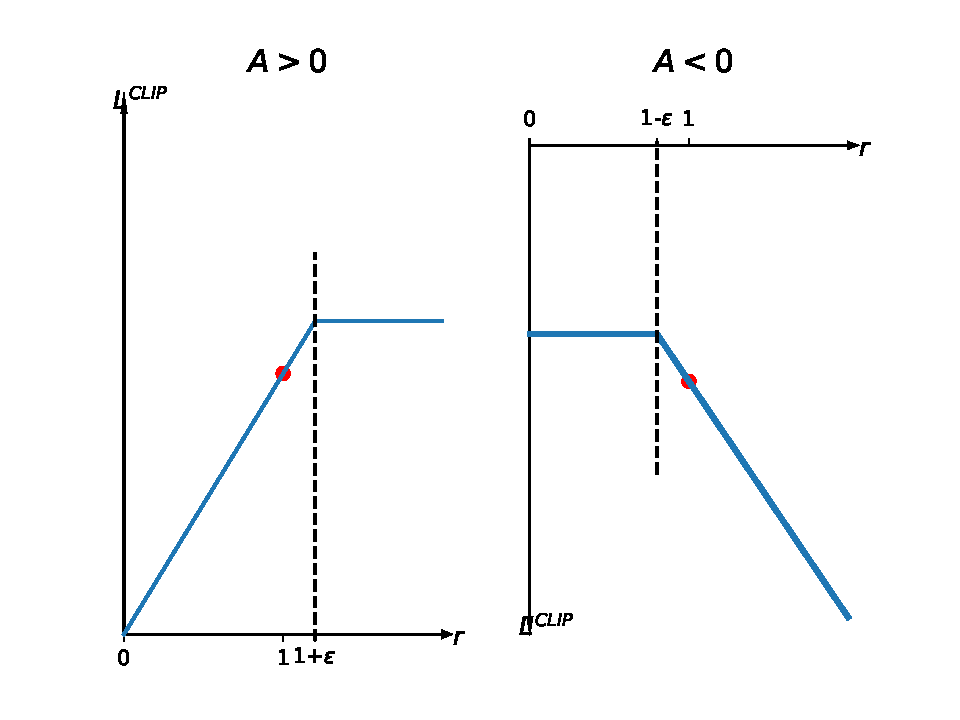
\includegraphics[height=0.5\textwidth, width=0.9\textwidth]{abbildungen/L_clip.pdf}
  \caption{Die Abbildung zeigt das Verhalten von $L^{CLIP}$ für einen einzelnen Zeitschritt $t$. Links ist der Fall $A > 0$ dargestellt, rechts der Fall $A < 0$.}
  \label{fig_L_clip}
\end{figure}

Zur Schätzung der Advantage Funktion kann eine abgeschnittene Form der Generalized Advantage Estimation verwendet werden. Diese Methode wurde von J. Schulman et. al. im Jahr 2016 publiziert \cite{GAE}. Sie bietet in gewisser Weise die Möglichkeit, die Varianz und den Bias des Schätzers zu regulieren. Dazu verwendet dieser die folgende Gleichung:

\begin{equation}
  \hat{A}_t = \delta_t + (\lambda \gamma) \delta_{t+1} + (\lambda \gamma)^2 \delta_{t+2} + \dots + (\lambda \gamma)^{T-t+1} \delta_{T-1} \qquad \text{mit } \delta_t = R_t + \gamma \hat{V}(s_{t+1}) - \hat{V}(s_t)
  \label{eq_gae}
\end{equation}

Dabei ist $\gamma$ wie gehabt der discount Faktor, $R_t$ der Reward im Zeitschritt t und $\hat{V}$ ist die geschätzte State-Value Funktion. Der Parameter $\lambda \in [0, 1]$ regelt das Verhältnis zwischen Bias und Varianz des Schätzers. Für die Randwerte von $\lambda$ ergeben sich folgende Spezialfälle. Für $\lambda = 0$ ergibt sich aus Gleichung \ref{eq_gae} die sogenannte Einschritt Temporal Difference, welche überlichweise einen Bias aufweist, allerdings keine Varianz. Für $\lamba = 1$ entspricht Gleichung \ref{eq_gae} der eines Monte Carlo Schätzers. Dieser weißt zwar keinen Bias auf, dafür aber eine hohe Varianz. Zusammenfassend ergibt sich, dass der Schätzer für $\lambda = 0$ varianzfrei ist und für $\lambda = 1$ biasfrei.

Viele Verfahren zur varianzreduzierten Schätzung der Advantage Funktion benutzen eine erlernte State-Value Funktion. Wenn darüber hinaus als Modell ein Neuronales Netzwerk verwendet werden soll, das geteilte Parameter für die Policy und die State-Value Funktion besitzt, muss die finale Verlustfunktion eine Kombination der zuvor präsentierten Verlustfunktion \eqref{L_CLIP} und eines auf der Value function basierenden Fehlers sein. Somit ergibt sich die folgende finale Verlustfunktion, die noch um einen Entropy-Bonus erweitert wurde, um eine ausreichende Exploration sicherzustellen:

\begin{equation}
	L_t^{CLIP+VF+S}(\theta) = \hat{\mathbb{E}}_t[L_t^{CLIP}(\theta) - c_1 L_t^{VF}(\theta) + c_2 S[\pi_\theta(s_t)]]
  \label{L_gesamt}
\end{equation}

Dabei sind $c_1$ und $c_2$ skalare Koeffizienten zur Gewichtung der einzelnen Terme. Der Term $L_t^{VF}$ ist die Verlustfunktion der geschätzten State-Value Funktion. Diese ist über den quadratischen Fehler $(V_\theta(s_t) - V_t^{targ})^2$ definiert.

Eine beispielhafte Implementierung eines \ac{PPO} Algorithmus, der Trajektorien fester Länge verwendet, wird nachstehend gezeigt. Dabei werden in jeder Iteration von jedem Actor zunächst über $T$ Zeitschritte Daten gesammelt, indem auf der Policy basierend Aktionen ausgeführt werden und die so entstehenden Trajektorien aufgezeichnet werden. Danach wird auf Basis dieser die Advantage Funktion geschätzt. Abschließend wird für alle zuvor gesammelten Daten die Verlustfunktion \eqref{L_gesamt} berechnet und optimiert, d.h. es wird es wird ein Gradientenschritt getätigt. Dazu werden die Daten in Minibatches der Größe $M<NT$ unterteilt, die wiederum für $K$ Epochen zum Training verwendet werden.

\begin{algorithm}
	\caption{\ac{PPO}, Actor-Critic Style}
	\begin{algorithmic}
		\For{$iteration=1,2,\dots$}
			\For{$actor=1,2,\dots,N$}
        \State Führe die Policy $\pi_{\theta_{old}}$ in der Umgebung für T Zeitschritte aus
				\State Berechne eine Schätung der Advantage function $\hat{A}_1,\dots,\hat{A}_T$
			\EndFor
			\State Optimiere $L^{CLIP+VF+S}$ bezüglich $\theta$ für $K$ Epochen und einer Minibatch Größe $M<NT$
			\State $\theta_{old} \gets \theta$
		\EndFor
	\end{algorithmic}
\end{algorithm}


\section{Neural Map}
\label{sec_neural_map}

Nachdem im vorangegangen Abschnitt mit dem \ac{PPO} Algorithmus eine Möglichkeit zum Trainieren einer entsprechend parametrisierten Policy gegeben wurde, soll im folgenden Abschnitt das im Rahmen dieser Arbeit hierfür verwendete Modell, die Neural Map, vorgestellt werden. Diese wurde von E. Parisotto und R. Salakhutdinov im Jahr 2018 veröffentlicht \cite{NeuralMap}. Es handelt sich bei der Neural Map um ein vollständig differenzierbares Modell zur Paremtrisierung einer Policy, das über einen externen Speicher mit trainierbarem Lese- und Schreiboperator verfügt.

Speicher bzw. ein Gedächtnis sind eine entscheidende Komponente, um einem Agenten sinnvolles Handeln zu ermöglichen. Ohne diese Komponente kann der Agent sein Verhalten nur durch seine aktuelle Wahrnehmung steuern und ist somit nicht in der Lage, längerfristige Pläne umzusetzen. Modelle, die externe Speicher verwenden, können im Wesentlichen in zwei Kategorien unterschieden werden, solche mit einem trainierbarem Schreiboperator und solche ohne einen. Zweitere haben für gewöhnlich eine feste Speichergröße. Ein solches Modell kann z.B. die letzten $N$ durch den Agenten beobachteten Zustände speichern. Da es aufgrund des nicht trainierbaren Schreiboperators nicht lernt, welche Informationen gespeichert werden sollen, lernt es, wie es auf den Speicher zugreifen muss. Dieser Ansatz besitzt jedoch zwei Nachteile. Zum einen kann der Speicher beliebig viele redundante Informationen enthalten. Zum anderen muss die Größe des Speichers geeignet gewählt werden, was in der Regel a priori Wissen über die Aufgabe des Agenten voraussetzt. Hat der Agent für seine aktuelle Aufgabe z.B. eine maximale Anzahl an Schritten vorgegeben, so sollte $N$ größer sein als diese. Modelle mit trainierbaren Schreiboperatoren sind potentiell leistungsfähiger, da sie erlernen können, welche Informationen sie speichern sollen und welche sie ignorieren. Sie benötigen somit kein a priori Wissen darüber, was sie speichern sollen und können Informationen für eine beliebige Zeitdauer speichern. Basierend auf dem zweiten Ansatz, d.h. einem Modell mit externem Speicher und trainierbarem Schreiboperator, entwickelten die Autoren die Neural Map, deren detailierte Struktur im Folgenden präsentiert wird.

Die Neural Map wurde für den Einsatzzweck entworfen, dass der Agent sich in einer 2- oder 3-dimensionalen Umgebung befindet. Während jeder Interaktion mit der Umgebung wird auf den internen Speicher zugegriffen in Form einer Leseoperation und einer anschließenden Schreiboperation. Dabei ist die Schreiboperation lokal beegrenzt, sodass nur die Stelle des internen Speichers beschrieben werden kann, die mit der aktuellen Position des Agenten in der Umgebung korrespondiert. Für die Einfachheit sei im Folgenden angenommen, dass sich der Agent in einer planaren Umgebung befindet, d.h. das sich seine Position in selbiger durch eine $x$- und eine $y$-Koordinate beschreiben lässt. Darüber hinaus wird angenommen, dass eine Koordinatentransformation $\psi(x,y)$ existiert. Diese bildet jede Postion $(x,y)$ des Agenten auf eine Speicherposition $(x',y')$ der Neural Map ab, wobei $x' \in \{0, \dots, W-1\}$ und $y' \in \{0, \dots, H-1\}$. Zur Vereinfachung der Notation seien im Folgenden alle Koordinaten durch $\psi$ in den Wertebereich zulässiger Speicherpositionen der Neural Map transformiert worden.

Der interne Speicher $M$ der Neural Map ist ein $C \times H \times W$ Feature Block. Dabei ist $C$ die Feature Dimension, $H$ ist die vertikale Größe und $W$ die horizontale Größe. Somit ist an jeder Position von $M$ ist ein $C$-dimensionales Feature gespeichert. Es ist $s_t$ der aktuelle Zustand, $M_t$ der aktuelle interne Speicher der Neural Map und $(x_t,y_t)$ die aktuelle Position des Agenten. Dann wird die Neural Map durch folgende Gleichungen beschrieben:

\begin{equation*}
  \begin{align*}
    r_t=read(M_t)&, \quad c_t=context(M_t, s_t, r_t), \\
    w_{t+1}^{(x_t,y_t)}=write(s_t, r_t, c_t, M_t^{(x_t,y_t)})&, \quad M_{t+1}=update(M_t, w_{t+1}^{(x_t,y_t)}), \\
    o_t=[r_t, c_t, w_{t+1}^{(x_t,y_t)}]&, \quad \pi_t(a|s)=\text{Softmax}(f(o_t))
  \end{align*}
\end{equation*}

Dabei ist $w_t^{(x_t,y_t)}$ das Feature an der Position $(x_t,y_t)$ zum Zeitpunkt $t$. Die Verkettung von Vektoren wird durch $[x_1, \dots, x_k]$ symbolisiert. Die Ausgabe der Neural Map zum Zeitpunkt $t$ durch durch $o_t$ gekennzeichnet. Diese wird anschließend von einem weiteren Neuronalen Netz $f$ verarbeitet, um die Policy $\pi(a|s)$ zu generieren. Die zuvor aufgestellten Gleichungen bzw. die damit korrespondierenden Operationen sollen nun ausführlicher erklärt werden.

\textbf{Global Read Operation:} Innerhalb der $read$ Operation durchläuft die aktuelle Neural Map $M_t$ ein Convolutional Neural Network, welches einen $C$-dimensionalen Feature-Vektor $r_t$ als Output generiert. Dieser Global Read Vektor $r_t$ kann als eine Zusammenfassung aller in der Neural Map gespeicherten Informationen angesehen werden. \\[0.1in]
\textbf{Context Read Operation:} Durch die $context$ Operation wird überprüft, ob gewisse Informationen bereits in der Neural Map vorhanden sind. Dazu werden zunächst der aktuelle Zustand $s_t$ und der aktuelle Global Read Vektor $r_t$ miteinander verkettet und mit einer Gewichtsmatrix $W$ multipliziert, um einen Query Vektor $q_t$ zu erhalten. Anschließend wird das Skalarprodukt des Query Vektors $q_t$ und jedes Feature Vektors der Neural Map M_t^{(x,y)} gebildet. Die auf diese Weise entstandenen Werte $a_t^{(x,y)}$ beschreiben die Ähnlichkeit der beiden zuvor miteinander verrechneten Vektoren. Als Nächstes werden diese Werte normalisiert, um eine Wahrscheinlichkeitsverteilung $\alpha_t^{(x,y)}$ über alle Positionen der Map zu generieren. Basierend auf dieser wird abschließend der gewichtete Durchschnitt aller Feature Vektoren $M_t^{(x,y)}$ berechnet, welcher im Weiteren auch als Context Read Vektor $c_t$ bezeichnet wird. Die zuvor beschriebenen Berechnungen lassen sich mit den folgenden Gleichungen zusammenfassen:
\begin{equation*}
  \begin{align*}
    q_t = W [s_t, r_t]&, \quad a_t^{x,y} = q_t \cdot M_t^{(x,y)}, \\
    \alpha_t^{(x,y)} = \frac{e^{a_t^{(x,y)}}}{\sum_{(w,z)} e^{a_t^{w,z}}}&, \quad c_t = \sum_{(x,y)} \alpha_t^{(x,y)} M_t^{(x,y)}
  \end{align*}
\end{equation*}
Die Context Read Operation ermöglicht es der Neural Map als eine Art assoziativer Speicher zu fungieren. Dazu übergibt der Agent einen mitunter unvollständigen Speicher, den Query Vektor $q_t$, an die Operation und diese gibt ihm den vervollständigten Speicher zurück, der widerum $q_t$ am ähnlichsten ist. Somit kann der Agent beispielsweise abfragen, ob er etwas zu seiner aktuellen Beobachtung Ähnliches bereits gesehen hat. \\[0.1in]
\textbf{Local Write Operation:} Die $write$ Operation generiert für die aktuelle Position des Agenten $(x_t,y_t)$ zum Zeitpunkt $t$ den $C$-dimensionalen Write Vektor $w_{t+1}^{(x_t,y_t)}$. Dazu erhält sie als Eingabe den aktuellen Zustand $s_t$, den aktuellen Global Read Vektor $r_t$, den aktuellen Context Read Vektor $c_t$ und den aktuellen Feature Vektor $M_t^{(x_t,y_t)}$ an der Position $(x_t.y_t)$. Diese Vektoren werden miteinander verkettet und anschließend von einem Neuronalen Netz $f_w$ verarbeitet, um den Write Vektor zu erzeugen, d.h. $w_{t+1}^{(x_t,y_t)} = f_w([s_t, r_t, c_t, M_t^{(x_t,y_t)}])$. Dieser Write Vektor fungiert als Schreibkandidat an der aktuellen Position $(x_t, y_t)$ \\[0.1in]
\textbf{GRU-based Local Write Operation:} Der zuvor beschriebene $write$ Operator generiert mit einem Neuronalen Netz den Write Vektor, mit welchem dann das Feature des internen Speichers an der entsprechenden Position einfach hart überschrieben wird. Alternativ zu diesem Vorgehen kann eine Schreiboperation verwendet werden, die von der sogenannten Gated Recurrent Unit inspiriert wurde. Diese berücksichtigt das zuvor an der entsprechenden Position gespeicherte Feature bei der Berechnung des neuen Write Vektors. Solche Schreiboperationen verfügen über eine lange Geschichte im Bereich rekurrenter Neuronaler Netze und haben in diesem Bereich ihre Fähigkeit zum Speichern von Informationen über einen langen Zeitraum schon oft unter Beweis gestellt. Die GRU-basierte Schreiboperation wird durch die folgenden Gleichungen definiert:

\begin{equation*}
  \begin{align*}
    r_{t+1}^{(x_t,y_t)} &= \sigma(W_r[s_t, r_t, c_t, M_t^{(x_t,y_t)}]) \\
    \hat{w}_{t+1}^{(x_t,y_t)} &= \tanh (W_{\hat{h}}[s_t, r_t, c_t] + U_{\hat{h}}(r_{t+1}^{(x_t,y_t)} \odot M_t^{(x_t,y_t)})) \\
    z_{t+1}^{(x_t,y_t)} & = \sigma(W_z[s_t, r_t, c_t, M_t^{(x_t,y_t)}]) \\
    w_{t+1}^{(x_t,y_t)} &= (1 - z_{t+1}^{(x_t,y_t)}) \odot M_t^{(x_t,y_t)} + z_{t+1}^{(x_t,y_t)} \odot \hat{w}_{t+1}^{(x_t,y_t)}
  \end{align*}
\end{equation*}
Dabei kennzeichnet $x \odot y$ das Hadamard-Produkt der Vektoren $x$ und $y$, d.h. die elementweise Multiplikation. Bei $W_*$ und $U_*$ handelt es sich um Gewichtsmatrizen. $\sigma(\cdot)$ ist die Sigmoidfunktion, die definiert ist als $\sigma(x) = \frac{1}{1+e^{-x}}$. In Anlehnung an die GRU-Terminologie wird $r_{t+1}^{(x_t,y_t)}$ als Reset Gate und $z_{t+1}^{(x_t,y_t)}$ als Update Gate bezeichnet. Diese beiden steuern, wie stark sich der neue Write Vektor $w_{t+1}^{(x_t,y_t)}$ von dem alten Feature an der entsprechenden Position des internen Speichers unterscheidet.\\[0.1in]
\textbf{Map Update Operation:} Für den nächsten Zeitschritt $t+1$ wird die dazugehörige Neural Map $M_{t+1}$ durch die $Update$ Operation erzeugt. Dabei ist die aktualisierte Neural Map $M_{t+1}$ bis auf an der Position des Agenten $(x_t,y_t)$ gleich der vorangegangenen Neural Map $M_t$. An dieser Position wurde der zuletzt generierte Write Vektor $w_{t+1}^{(x_t,y_t)}$ gespeichert, sodass sich die $Update$ Operation durch die folgende Gleichung beschreiben lässt:
\begin{equation*}
  \begin{align*}
    M_{t+1}^{(a,b)} =
    \begin{cases}
      w_{t+1}^{(x_t,y_t)}, & \quad \text{für} (a,b) = (x_t,y_t) \\
      M_t^{(a,b)}, & \quad \text{für} (a,b) \ne (x_t,y_t)
    \end{cases}
  \end{align*}
\end{equation*}

Die Abbildung \ref{fig_neural_map} gibt eine Übersicht über das Wechselspiel zwischen den einzelnen Operatoren und den daraus resultierenden Datenpfaden. Auf der linken Seite finden sich mit dem aktuellen Zustand des internen Speichers $M_t$ und dem aktuellen Zustand der Umgebung $s_t$ die Eingaben der Neural Map im Zeitschritt $t$. Anhand den von hier ausgehenden Pfeilen ist ersichtlich, in welche Operationen wiederum diese Als Eingabe eingehen. Entsprechendes gilt für die Ausgangspfeile auf der rechten Seite der jeweiligen Operatoren. Der gestrichtelte Pfeil deutet an, dass das Feature $M_t^{(x_t,y_t)}$ ein Teil des gesamten internen Speichers $M_t$ ist und somit aus diesem extrahiert werden kann. Verzweigungen der Datenpfade sind durch die schwarz ausgefüllten Kreise dargestellt. Auf der rechten Seite sind mit der Policy $\pi(a|s)$ und dem Folgezustand des internen Speichers $M_{t+1}$ die Ausgaben der Neural Map im Zeitschritt $t$ angegeben.


\begin{figure}[ht!]
  \centering
  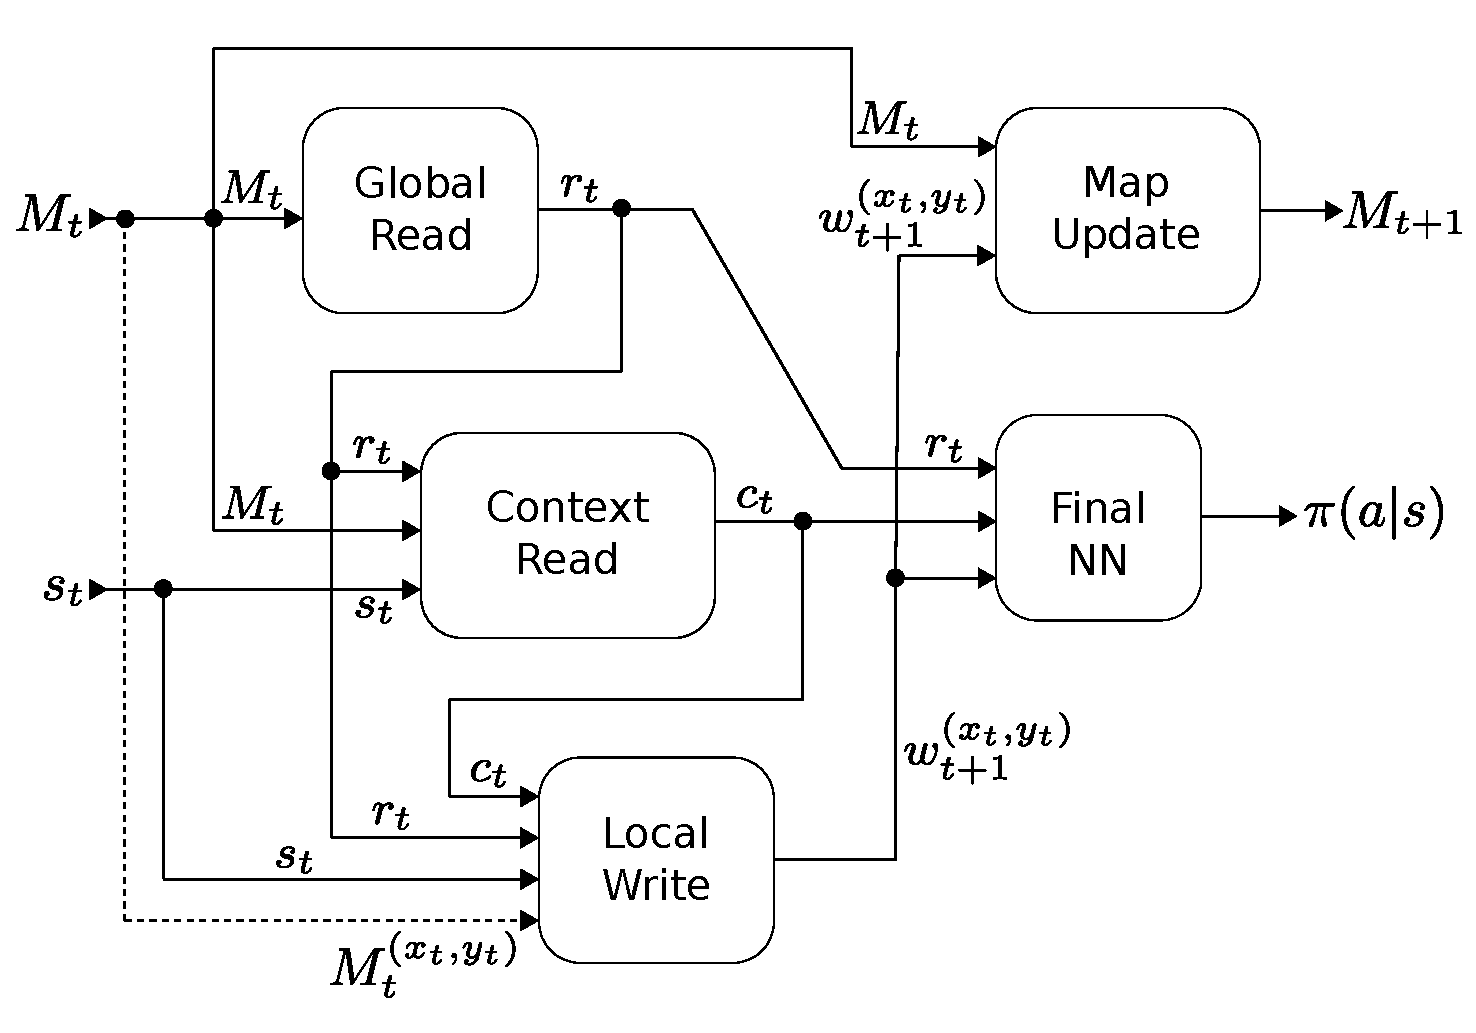
\includegraphics[keepaspectratio,width=0.75\textwidth]{abbildungen/neural_map.pdf}
  %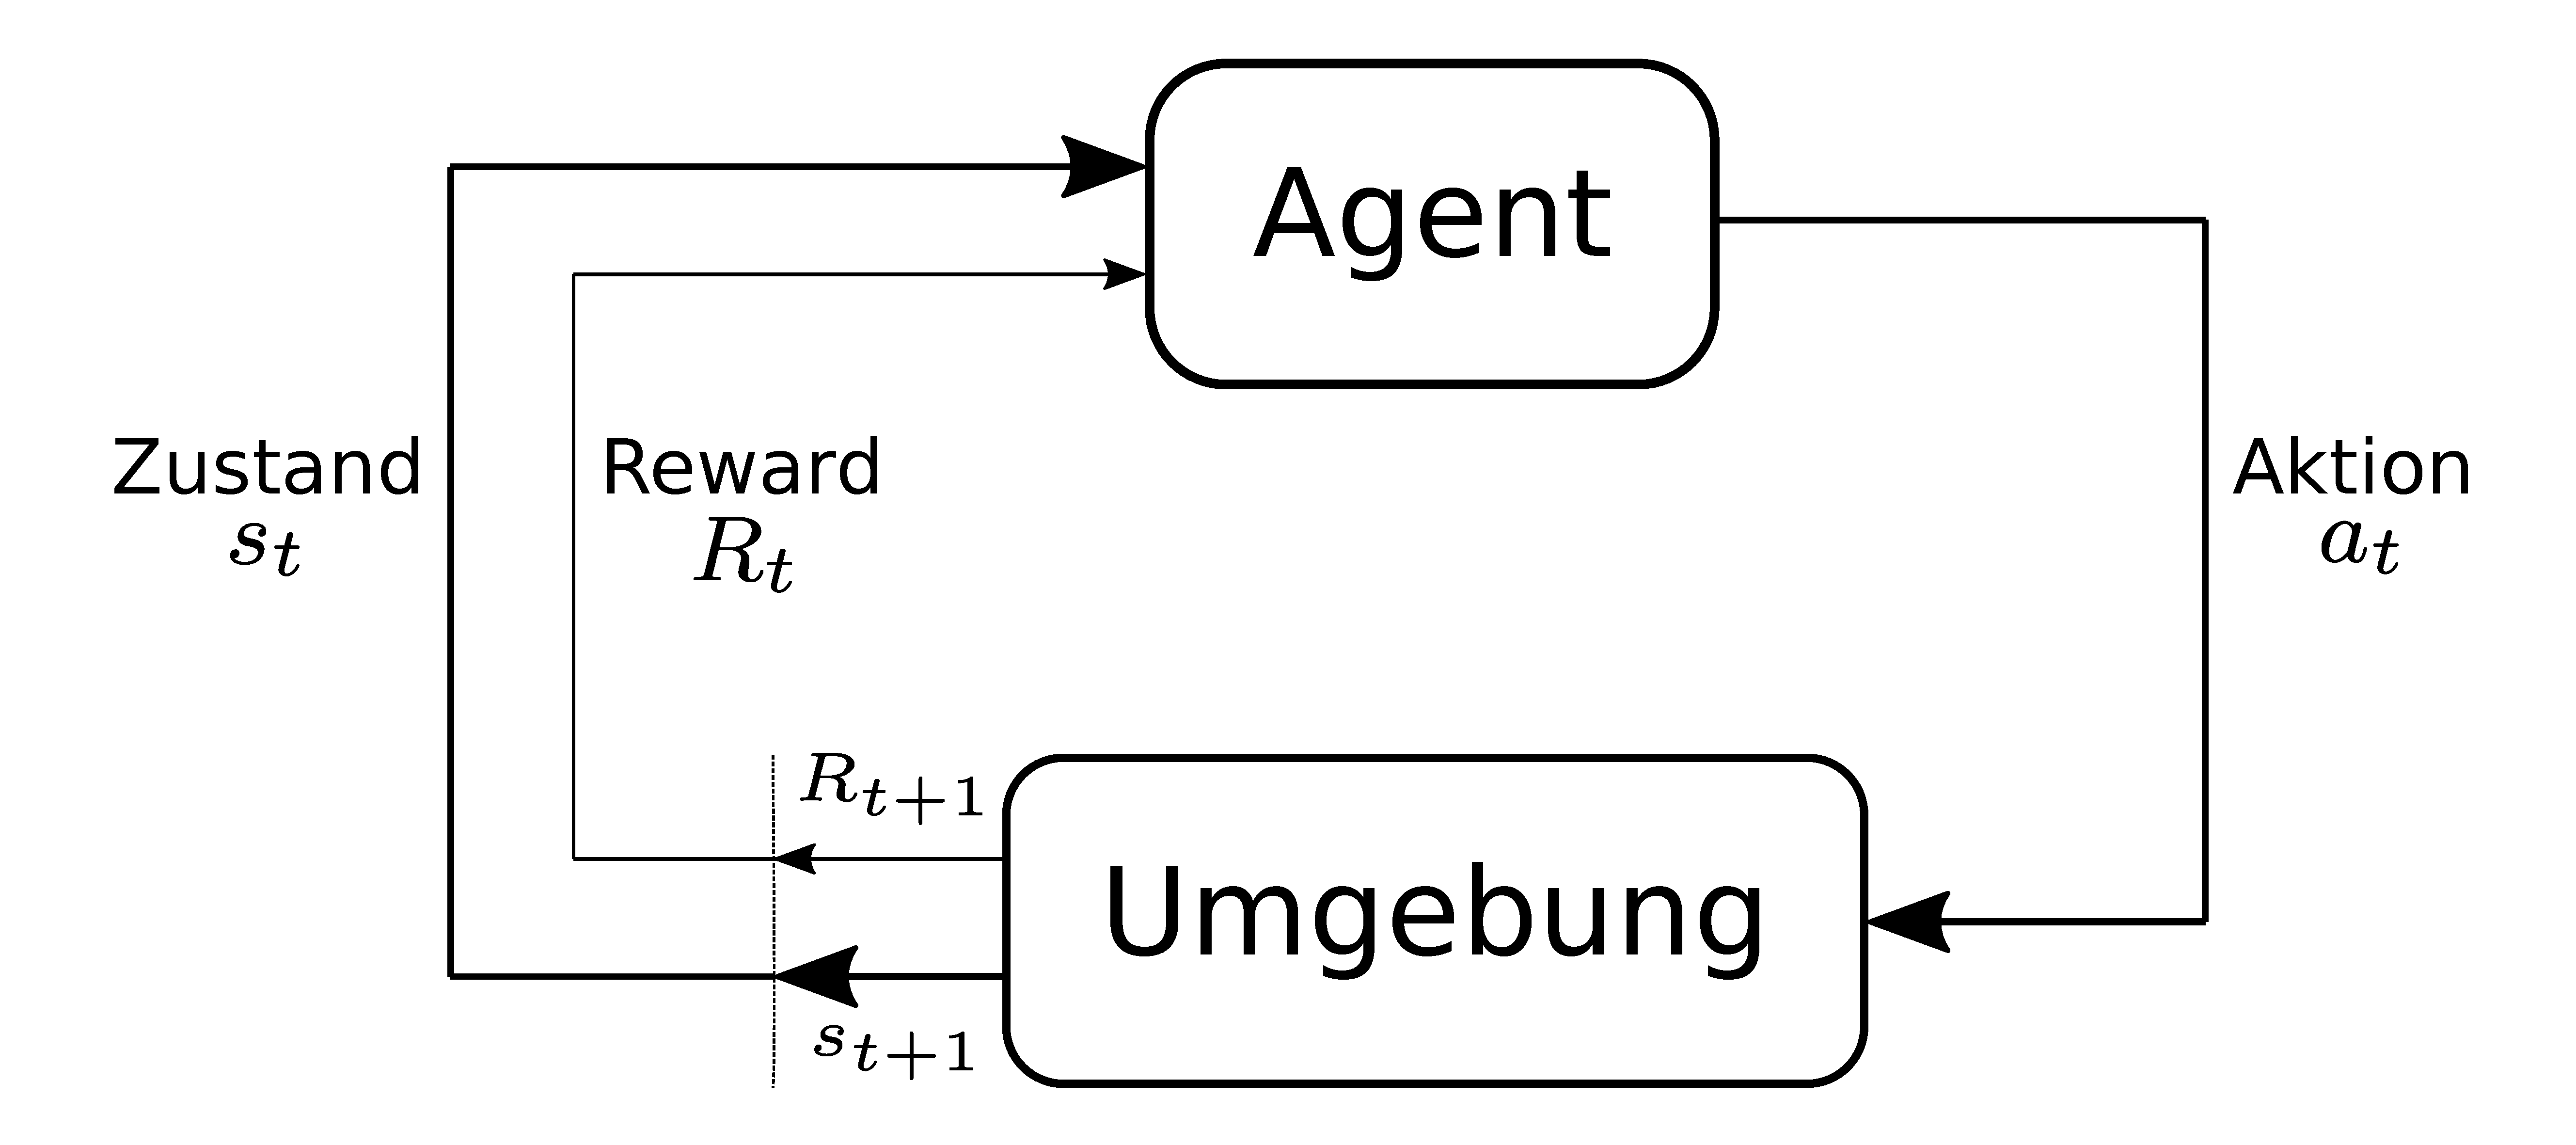
\includegraphics[height=0.5\textwidth, width=0.9\textwidth]{abbildungen/schnittstelle_agent_umgebung.pdf}
  \caption{Die Abbildung zeigt das Wechselspiel zwischen den verschiedenen Operatoren und die sich daraus ergebenen Datenpfade. Auf der linken Seite befinden sich mit $s_t$ und $M_t$ die Eingaben der Neural Map und auf der rechten Seite mit $\pi(a|s)$ und $M_{t+1}$ die Ausgaben. Die Wege dazwischen können anhand der Pfeile nachvollzogen werden.}
  \label{fig_neural_map}
\end{figure}


\section{Long short-term memory}
\label{sec_lstm}

Zum Abschluss dieses Kapitels wird eine kurze Einführung in das sogenannte Long Short-Term Memory (LSTM) gegeben. Es handelt sich bei dem LSTM um eine Architektur für ein rekurrentes Neuronales Netz, die von S. Hochreiter und J. Schmidhuber im Jahr 1997 publiziert wurde \cite{LSTM}. Im Jahr 1999 erhielt sie durch F. Gers et. al. noch eine entscheidende Erweiterung, wodurch der heute gebräuchliche Aufbau des LSTM entstand \cite{ForgetGate}. Besondere Anwendung findet das LSTM üblicherweise in der Analyse von Zeitreihen, es lässt sich aber auch zur Parametrisierung einer Policy im RL Kontext verwenden. Da es durch seine rekurrente Struktur in der Lage ist, Informationen über einen beliebigen Zeitraum zu speichern, dient das LSTM wie bereits im Neural Map Paper für die im Rahmen dieser Arbeit durchgeführten Experimente als Referenz.

Die entscheidende Komponente des LSTM zum Speichern von Informationen ist der Zellzustand $c_t$. Unter Verwendung mehrerer sogenannter Gates, namentlich des Forget Gates $f_t$, des Input Gates $i_t$ und des Output Gates $o_t$, wird der Datenfluss des Zellzustandes von einem zum nächsten Zeitschritt gesteuert. Jedes Gate erhält die Eingabe des LSTM $x_t$ und die vorherige Ausgabe des LSTM $h_{t-1}$ und berechnet daraus unter Verwendung eines Fully Connected Layers mit Sigmoid-Aktivierungsfunktion seine Ausgabe. Auf die gleiche Weise wird die Zellaktivierung $\hat{c}_t$ berechnet, allerdings wird hierbei $tanh$ als Aktivierungsfunktion verwendet. Der Zellzustand $c_t$ ergibt sich dann aus der Summe der Hadamard-Produkte von $f_t$ und $c_{t-1}$ und  $i_t$ und $\hat{c}_t$. Innerhalb dieser Summe reguliert das Forget Gate $f_t$, wie viel des vorherigen Zellzustandes $c_{t-1}$ vergessen bzw. übernommen wird. Über das Input Gate $i_t$ wird gesteuert, wie stark die aktuelle Zellaktivierung $\hat{c}_t$ berücksichtigt wird. Diese kann als Schreibkandidat für den Zellzustand angesehen werden. Anschließend kann die Ausgabe des LSTM $h_t$ berechnet werden aus dem Hadamard-Produkt von $o_t$ und dem Tangens hyperbolicus von $c_t$. Auf diese Weise bestimmt das Output Gate, in welchem Maße der Zellzustand in die Ausgabe des LSTM mit eingeht. Die zuvor beschriebene Struktur bzw. die Operationen können mit den folgenden Gleichungen zusammengefasst werden:

\begin{equation*}
\begin{align*}
	f_t &= \sigma(W_f x_t + U_f h_{t-1} + b_f) \\
	i_t &= \sigma(W_i x_t + U_i h_{t-1} + b_i) \\
	o_t &= \sigma(W_o x_t + U_o h_{t-1} + b_o) \\
	\hat{c}_t &= tanh(W_c x_t + U_c h_{t-1} + b_c) \\
	c_t &= f_t \odot c_{t-1} + i_t \odot \hat{c}_t \\
	h_t &= o_t \odot tanh(c_t)
\end{align*}
\end{equation*}

Dabei ist $\sigma(\dots)$ die Sigmoid-Funktion. Bei $W_*$ und $U_*$ handelt es sich um Gewichtsmatrizen und bei $b_*$ um Bias-Vektoren. Das Hadamard-Produkt zweier Vektoren wird durch $\odot$ gekennzeichnet.
